% !TEX TS-program = xelatex
% !TEX encoding = UTF-8 Unicode
% !Mode:: "TeX:UTF-8"
%\documentclass{article}
%\documentclass[10pt,aps,showpacs,preprintnumbers,amsmath,amssymb,prl,twocolumn]{revtex4-1}
%\documentclass[10pt,aps,showpacs,preprintnumbers,amsmath,amssymb,prl]{revtex4-1}

%\documentclass{jfm_revised}
\documentclass[10pt,aps]{article}

\usepackage{color,hyperref}
\usepackage{graphicx}
\usepackage{amssymb}
%RV\usepackage{/Users/lohsed/Documents/papers/sty-files/citesort}
%\usepackage{citesort}  % replace above
%\usepackage{subfigure,comment}
\usepackage{CN_Adobe_Fonts} 


%\usepackage{linespacing_fix} % disable extra space before next section
%\usepackage{natbib} 
\usepackage{epsfig}
\usepackage{fancyhdr}
\usepackage{color}
%\usepackage[normalmargins,normalleading,normalsections,normaltitle,normalindent,normalfloats]{savetrees}
\usepackage{url}

\language0


%\textheight240mm
%\textwidth155mm
%\oddsidemargin5mm
%\evensidemargin5mm
%\topmargin-10mm

\sloppy
\tolerance10000
\renewcommand{\baselinestretch}{1.0}

%%%%%%%%%%%%%%%%%%%%%%%%%%%%%%%%%%
%own text settings              %  ERC settings
\setlength{\textwidth}{17.3cm}  %17.3
 \setlength{\textheight}{23.5cm}  % 25.5
\setlength{\oddsidemargin}{-0.3cm} % -0.3
\setlength{\evensidemargin}{-0.3cm} % -0.3
 \setlength{\headheight}{0.0cm}
% \setlength{\topmargin}{-1.6cm}   % -1.8
 \setlength{\topmargin}{-1.6cm}   % -1.8
 
\newenvironment{packed_item}{
\begin{itemize}
  \setlength{\itemsep}{1pt}
  \setlength{\itemsep}{0pt} % eventual weg
  \setlength{\parskip}{0pt}
  \setlength{\parsep}{0pt}
}{\end{itemize}}




%%%%%%%%%%%%%%%%%%%%%%%%%%%%%%%%

\pdfpagewidth 8.2in
\pdfpageheight 12 in 
%\pagestyle{fancy}
\headheight 20pt 
\pagestyle{plain}
%\lhead{Lohse}
%\rhead{PhysBoil}
\linespread{1.5} % set the line spacing 




\newcommand\euro{{\sffamily C%
    \makebox[0pt][l]{\kern-.70em\mbox{--}}%
    \makebox[0pt][l]{\kern-.68em\raisebox{.25ex}{--}}}}


\setcounter{totalnumber}{10}

\newcommand{\ageq}{\mbox{\
\raisebox{-.9ex}{$\stackrel{\textstyle >}{\sim}$}\ }}



\def\be{\begin{equation}}
\def\ee{\end{equation}}

\def\gtwid{\mathrel{\raise.3ex\hbox{$>$\kern-.75em\lower1ex\hbox{$\sim$}}}}
\def\alt{\mathrel{\raise.3ex\hbox{$<$\kern-.75em\lower1ex\hbox{$\sim$}}}}

\def\agt{\mathrel{\raise.3ex\hbox{$>$\kern-.75em\lower1ex\hbox{$\sim$}}}}

\def\Ra{\textrm{Ra}}
\def\Pr{\textrm{Pr}}


\newcommand{\bea}{\begin{eqnarray}}
\newcommand{\eea}{\end{eqnarray}}
\newcommand{\pat}{\partial}
\newcommand{\del}{\nabla}

\newcommand{\mar}[1]{\marginpar{\footnotesize{\textcolor{red}{#1}}}} % commentaire en marge
\newcommand{\red}[1]{{\textcolor{red}{#1}}} % commentaire en rouge

\newcommand\remark[1]{{\footnotesize \color{green}Comment: #1}}

\def\gtwid{\mathrel{\raise.3ex\hbox{$>$\kern-.75em\lower1ex\hbox{$\sim$}}}}
\def\alt{\mathrel{\raise.3ex\hbox{$<$\kern-.75em\lower1ex\hbox{$\sim$}}}}

\def\agt{\mathrel{\raise.3ex\hbox{$>$\kern-.75em\lower1ex\hbox{$\sim$}}}}

\def\x{{\mbox{\boldmath$x$}}}
\def\u{{\mbox{\boldmath$u$}}}
\def\r{{\mbox{\boldmath$r$}}}
\def\f{{\mbox{\boldmath$f$}}}
\def\q{{\mbox{\boldmath$q$}}}
\def\p{{\mbox{\boldmath$p$}}}
\def\k{{\mbox{\boldmath$k$}}}
\def\n{{\mbox{\boldmath$n$}}}
\def\g{{\mbox{\boldmath$g$}}}
\def\v{{\mbox{\boldmath$v$}}}
\def\V{{\mbox{\boldmath$V$}}}
\def\U{{\mbox{\boldmath$U$}}}
\def\nab{{\mbox{\boldmath$\nabla$}}}



\def\ni{{\noindent}}
\def\eps{{\epsilon}}
%\def\fns{{\footnotesize}}
\def\begineq{\begin{equation}}
\def\endeq{\end{equation}}
\def\rel{{Re_\lambda}}



\begin{document}


\section*{ \hskip 5cm {\color{blue}湍流热对流边界层转捩的实验研究}}
\vskip 6pt
%\noindent

\hskip 6cm  作者:黄海龙,顾姣燕,张玲,何晓舟 

{\hskip 2cm \small 单位:哈尔滨工业大学(深圳)机电学院湍流-噪声-振动耦合与控制研究所, 深圳邮编518005}

{\hskip 6cm \small 邮箱:huanghailong@stu.hit.edu.cn} 




% document context starts from here %


\vskip 1cm



\hskip 6pt {\bf 摘要}: 本论文将介绍国际湍流研究领域关于热对流系统中边界层由层流态向湍流态转捩的实验研究进展。最新的研究结果发现当普朗特数 $\Pr = 1$,边界层的转捩发生在$\Ra = 10^{14}$附近,符合``GL"理论模型关于Kraichnan``终极状态"的预测。边界层转捩之后,温度场的空间分布和统计性质遵守流体力学经典的湍流边界层``边壁法则"。研究湍流热对流边界层的转捩将有助于理解和揭示在更大湍流尺度下(如地球物理和天体物理系统中)热对流传热规律和内部湍流流动性质。
\vskip 24pt


\hskip 6pt {\bf 关键词}:湍流;热对流;湍流边界层;边壁法则



\vskip 1.5cm


\section*{1 国内外研究现状}
\vskip 6pt

{研究固定边界附近流场由层流态向湍流态转捩是湍流领域的经典问题之一 \cite{Rey1883},跟随流体力学 100 多年的发展,至今仍然是国际湍流研究领域的前沿热点课题,近十年的研究成果经常发表在 Nature、Science、Physical Review Letters 和流体力学顶级期刊上 \cite{SK16,SHG16,LSAJAH16,Ba16,BSMLAH15,AMRH13,AMLABH11,HLATS10,ESHW07}。由于在湍流热对流流场中同时存在速度和温度边界层,两者间的相互影响使得热对流边界层转捩问题更加复杂。著名理论物理学家 Robert Kraichnan 的理论模型\cite{Kr62}指出当对流系统内部流场湍流度 (用 Ra 数来表征) 不断增加并超过临界值,边界层最终会在剪切力和浮力的共同作用下由层流向湍流态(又被称为 Kraichnan``终极状态")转捩。大尺度自然对流系统(如大气对流、海 洋对流、恒星对流层等流场系统)\cite{Sp71}和大尺度工程对流系统(如:核电站降温塔等)理论上处于 “终极状态” , 而绝大多数实验数据和数值计算结果都远小于转捩临界点 \cite{AGL09,Ah09}。由于流场的能量传输和流动混合性质在边界 层转捩前后都将发生本质的变化,所以研究转捩何时发生以及处于 ``终极状态" 中的湍流性质不仅是研究地球物理和天体物理湍流系统的重要基础课题,也与许多大型工业生产设计密切相关。
\vskip 6pt

 对于封闭系统,``终极状态"的转捩点 Ra* 依赖于流场宽高比和工作流体的 Pr 数。对于两者数值均在 1 附近的 系统,GL理论模型\cite{GL00,GL01} 预测“终极状态”的转捩点发生在 $\Ra^* = 10^{14}$ 附近。因为绝大部分实验和数值模拟只能达到 $\Ra = 10^{12}$ 或以下, 所以对于 Kraichnan ``终极状态"的直接验证非常困难。为了提高 $\Ra$ 数,B\'ernard Castaing 在 Grenoble 的实验室使用低温氦气(5K)作为工作流体达到 $\Ra = 10^{16}$,实验结果发现“终极状态”的转捩点在 $\Ra = 10^{11}$ 附近,比理论值低三个数量级\cite{CCCHCC97,CCCCH01}。Katepalli R. Sreenivasan 在 Oregan 的研究组重复了该实验,并将 $\Ra$ 数提高到 $10^{17}$,实验结果没有发现转捩发生\cite{NSSD00}。值得注意的是受限于实验条件,这两组实验中的 $\Pr$ 数都没有得到精确的控制:前者改变了 4 倍,而后者改变了 100 倍。 如何在实验中达到高 $\Ra$ 数,同时保持 $\Pr$ 不变是验证湍流热对流 ``终极状态"的关键。
\vskip 6pt

Eberhard Bodenschatz和Guenter Ahlers在 G\"ottingen 的研究组使用室温 SF$_6$ 气体作为工作流体,通过将气体增压到 2 MPa 达到 $\Ra = 4 \times 10^{15}$ ,同时通过精确控制气体工作温度将 $\Pr$ 数控制在 $0.79 - 0.86$ 的极小范围内,排除了由流体 $\Pr$ 数变化而影响结论的可能。全套实验装置重 12 吨,使用气体总 重量 2000 公斤,温度控制和测量精度 0.005K。实验结果发现 Kraichnan ``终极状态"的转捩发生在$2 \times 10^{13} < \Ra < 5 \times 10^{14}$ \cite{HFNBA12,HFBA12,AHFB12},和理论预测\cite{GL01}十分吻合。


\section*{2 重要科学问题}

2.1 改变 Pr 数对湍流边界层转捩点 Ra* 的影响 


Pr数对边界层转捩点Ra*的影响的理论研究起始于21世纪初期Grossmann 和Lohse 提出的GL理论~\cite{GL00,GL01},该理论是通过RBC系统中能量耗散率($\epsilon_u$)和温度耗散率($\epsilon_\theta$)的表达式而建立起来的,即:
\be
\rm \epsilon_u=\frac{\nu^{3}}{L^4}(\rm Nu-1)Ra Pr^{-2}
\ee
\be
\epsilon_\theta=\kappa \frac{\Delta^2}{L^2}\rm Nu
\ee
\vskip 6pt

由于边界层区和块区对能量耗散率和温度耗散率均有贡献,且两者的物理本质是不一样的,因此可以将RBC 系统的参数空间(Ra-Pr)分解为4 个主要的区间(如图\ref{fig:GL_Theory}):区间\uppercase\expandafter{\romannumeral1}: $\epsilon_u$和$\epsilon_\theta$都由边界层区主导;区间\uppercase\expandafter{\romannumeral2}: $\epsilon_u$由块区主导,$\epsilon_\theta$由边界层区主导;区间\uppercase\expandafter{\romannumeral3}: $\epsilon_u$由边界层区主导,$\epsilon_\theta$由块区主导;区间\uppercase\expandafter{\romannumeral4}: $\epsilon_u$和$\epsilon_\theta$都由块区主导。根据Pr数的大小,又可以将它们分为高Pr数区间和低Pr数区间,分别用下标``u”和``l”表示。GL理论的前提条件是系统速度和温度边界层满足Prandtl-Blasius层流边界层假设,在此条件下边界层厚度满足$\lambda_u$ $\sim $LRe$^{-1/2}$。在边界层上的剪切力主要取决于大尺度环流的速度和边界层厚度,因此对应的剪切Re数可以表示为:
\be
\rm Re_s=\frac{U\lambda_u}{\nu}\sim \sqrt{Re}
\ee
\vskip 6pt

类似有壁面的剪切流流动,当Re$_s$不断增大至临界值时,层流边界层将向湍流边界层转捩,理论预测临界Re$_s$ = 420~\cite{LL63}。GL理论提出RBC系统只有在区间\uppercase\expandafter{\romannumeral2}和区间\uppercase\expandafter{\romannumeral4}才能达到足够大的
Re$_s$,相应的Pr和Ra$^*$之间存在以下关系:在区间\uppercase\expandafter{\romannumeral2}$_l$和区间\uppercase\expandafter{\romannumeral2}$_u$内,Ra$^* \sim $Pr$^{3/2}$;在区间\uppercase\expandafter{\romannumeral4}$_l$,Ra$^*\sim$ Pr$^1$。

\begin{figure}[htb]
  \centering
  \includegraphics[width=0.6\linewidth]{GL_Theory.pdf}
  \caption{GL理论(Ra-Pr)参数分区,大Pr数下的阴影区表示Re>50,小Pr下的阴影区表示Nu=1;虚线表示温度边界层厚度等于速度边界层厚度;点线表示转捩点Ra$^*$与Pr数的关系~\cite{GL00}}
  \label{fig:GL_Theory}
\end{figure}
\vskip 6pt


从实验中获得Pr对Ra$^*$的影响需要满足两个要求:一是使实验系统能达到足够大的Ra数,二是精确地控制Pr数的大小 。实验上主要通过两种方式来实现大Ra数,一种是用以接近汽–液临界点温度(约为5K)的高压氦气作为工作流体,另一种是用高压SF$_6$气体作为工作流体。采用低温氦气的原因是在接近汽-液临界温度时,氦气的动量扩散和温度扩散能力变弱即氦气的运动粘度$\nu$和热扩散率$\kappa$很小。根据Ra数的定义式,
\be
 Ra=\frac{\beta g\Delta L^3  }{\nu\kappa}
\ee
\vskip 6pt

其中$\beta$是等压热膨胀系数,g是重力加速度,$\Delta $是RBC上下板温差,L是上下板高度。从而在给定温差$\Delta$条件下,$\nu$和$\kappa$越小,所能达到的Ra数越大。Bernard Castaing实验组~\cite{CCCHCC97,CCCCH01}用低温氦气实验发现Ra$^*\approx 10^{11}$,比GL理论预测的10$^4$低三个数量级。Katepalli R. Sreenivasan 研究组重复该实验后却没有发现转捩点。出现这一矛盾结果可能是由两方面原因造成的:首先,在高Ra数下,低温氦气不满足Boussinesq 近似;其次,以接近汽–液临界点的高压氦气作为工作流体进行高Ra 数实验的过程中,氦气可能发生相变导致Pr急剧增大,从而导致Ra$^*$也急剧增大进而无法观察到转捩。
\vskip 6pt
采用高压SF$_6$能获得高Ra数则是因为对于气体~\cite{AFB09},

\be
\rm Ra=\frac{\beta g\Delta L^3 \rho^2 \emph C_p}{\lambda\mu}
\ee
\vskip 6pt

其中$\rho$是气体密度,$\mu$是动力粘度,$C_p$是定压比热容。在室温条件下工作气体远离汽化点,此时$\lambda$和$\mu$几乎不随压强$P$改变,而气体密度近似正比与$P$。因此在给定温差$\Delta$下,Ra $\sim\rho^2\sim P^2 M^2$(M是气体分子量),即Ra和$(MP)^2$成正比。Göttingen实验组~\cite{HFBA12}使用M=146 gmol$^{-1}$的SF$_6$气体当做工作流体,并将其加压到P=2 MPa从而实现了了极高的Ra数。通过精确控制Pr最后观察到了边界层的转捩,实验结果发现$2\times10^{13}$<Ra$^*$<$5 \times 10^{14}$,与GL理论预测的转捩点Ra$^*$相吻合。
\vskip 6pt

Jörg Schumacher实验组~\cite{SBPS16}用Pr=0.021的工作流体在$1.8 \times 10^3 \leq$ Re $\leq 4.6\times 10^6$下进行直接数值模拟,得到了系统的摩擦Re数与Ra数的关系,
\be
\rm Re_\tau=u_\tau\delta_*\sqrt{\frac{Ra}{Pr}}
\ee
\vskip 6pt

其中$u_\tau$表示无量纲摩擦速度。通过进一步分析,得到当Re$_\tau$=200时,$\Ra \simeq 10^{11}$,此时系统的层流边界层将向湍流过渡,数值模拟的数据得出$3\times 10^{10}\lesssim \Ra^* \lesssim 5\times 10^{11}$,即位于GL理论的\uppercase\expandafter{\romannumeral2}$_l$区间。利用GL~\cite{GL00}的预测:在\uppercase\expandafter{\romannumeral2}$_l$ 区间内,Ra$^* \sim $Pr$^{3/2}$,将直接数值模拟的计算结果外延到 Pr = 0.8,得到转捩点$\Ra^* = 2 \times 10^{13}$,与Göttingen 研究组在 Pr = 0.8 附近得到的实验结果非常吻合。类似地,用Göttingen实验组的数据及GL关于剪切雷诺数的模型~\cite{GL02}:Re$_s=a$Re$^1/2$,可以得到$\rm{Re^*}/{\emph a}$=562,进而推算出当Pr=0.021时,系统的转捩点Ra$^*=9.7\times10^{10}$,与DNS结果一致 。实验和数值计算的结果给出 $\Ra^* \sim \Pr^\alpha$,指数$\alpha$ 随$\Ra$ 数增大而增大。当 $\Ra \simeq 10^{13}$ 时 $\alpha = 1.43$~\cite{ABH17}。\\



2.2 边界层转捩前后热对流大尺度环流的动力学性质 

由于边界层的不稳定性产生的羽流在热对流流场中形成与系统尺度相当的大尺度环流。大尺度环流是湍流热对流流动的一个重要标志,也是内部流场热量流传输的快速通道。 在大尺度环流面内,热羽流总是沿着一侧上升,冷羽流总是沿着另一侧下沉,从而形成一个旋转的大尺度环流面。大尺度环流面具有两个特征速度:旋转角速度$\gamma$ \cite{QT01a}和进动角耗散速度 $\dot{\theta}$ \cite{BA06a}。根据这两个特征速度定义的无量纲雷诺数$Re_U \simeq 2UR/\nu$和$Re_{\dot{\theta}} \simeq 2\sqrt{D_\theta/\nu}$通常被用来描述大尺度环流的主要动力学性质。式中,$U = \gamma R$,${\theta}$ 和 R分别是大尺度环流的方向角和半径。
\vskip 6pt


在边界层发生湍流态转捩前后,大尺度环流的动力学性质也会发生相应的改变。最近的实验测量发现大尺度环流角向运动的动力学性质与 $\Ra$ 数的标度率在 $\Ra = 2 \times 10^{13}$ 附近发生转捩\cite{HBA16}。当$\Ra < \Ra_1^* = 2 \times 10^{13}$时,实验结果发现$Re_{\dot{\theta}} \sim \Ra^{0.28}$,与热对流``经典状态"下的结果相一致\cite{BA06a,BA06b}。当$\Ra > \Ra_2^* = 8 \times 10^{13}$时,实验结果发现新的标度率$Re_{\dot{\theta}} \sim \Ra^{0.4}$。在相同的热对流实验装置中实验还发现雷诺数$Re_U$有类似的转捩:当$\Ra < \Ra_1^* = 2 \times 10^{13}$时,$Re_U \sim \Ra^{0.42}$;当$\Ra > \Ra_2^* = 8 \times 10^{13}$时,$Re_U \sim \Ra^{0.5}$。在$\Ra_1^*<\Ra < \Ra_2^*$区间范围内,两个雷诺数均不符合单一标度率,表明系统正处于转捩过程中。
对大尺度环流动力学性质的测量分析,进一步证实热对流“终极状态”的存在。\\




2.3 边界层附近温度场的空间分布及其统计性质

湍流热对流边界层发生转捩之后,热对流系统从``经典状态''转变为Kraichnan``终极状态''。系统边界层附近温度场的空间分布及其统计性质也会发生相应的转变。
``经典状态''下,粘性边界层与热边界层共存,粘性边界层保持层流状态,但层流边界层内部存在一定涨落。定义无量纲的时间平均温度为:
\be
\Theta(z,r)=\frac{\langle T(z,r,t)\rangle-T_m}{\Delta T}
\ee


其中$r$是到中心线的距离,$z$是离开底板的垂直高度,$T_m$为平均温度,$\Delta T$为上下板温差。Göttingen研究组~\cite{ABFGHLSV12}\cite{ABH14}在Pr$\approx0.8$和Ra$=2×10^{12}$ 下的实验结果如图\ref{fig:LOW}所示:在垂直壁面方向上热边界层可分为内区和外区,内区又可细分为热底层、缓冲层和对数层。在热底层和缓冲层内,平均温度$\Theta(z)$与离开边壁的距离呈线性关系;在对数层,平均温度$\Theta(z)$与离开边壁的距离呈对数关系;而在外区,平均温度$\Theta(z)$整体上呈对数分布。这与剪切流动中著名的``边壁法则''(即湍流边界层附近的平均流线速度的对数分布率)十分类似,剪切流动中流线速度的对数分布来源于近壁面处的剪切不稳定性,剪切不稳定性导致了相关涡的形成,最终产生平均速度的对数分布关系。而在热边界层中 ,其平均温度对数分布不是由剪切流动产生的,而是来源于热边界层的不稳定性,这导致了羽流的形成,最终形成平均温度的对数分布。
\begin{figure}[ht]
  \centering
  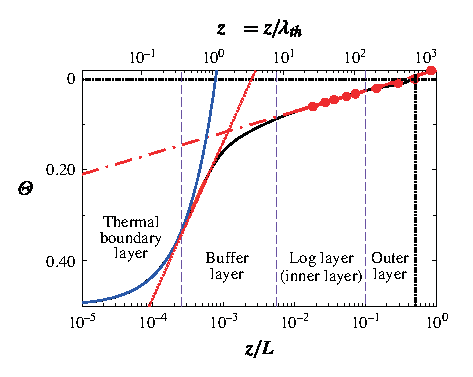
\includegraphics[width=0.7\linewidth]{LOW.eps}
  \caption{经典状态下边界层处无量纲平均温度分布~\cite{ABH14}}
  \label{fig:LOW}

\end{figure}
实验发现,靠近上板和下板的对数温度分布分别为$\Theta=\rm A(r)ln⁡(z⁄L)+B(r)$和$\Theta=\rm A'(r)ln⁡(1-z⁄L)+B(r)$,其中A和$A'$为对数项的振幅大小,B为与r相关的参数。经典状态下,上下板边界层温度分布关于中心镜像对称且振幅—A与$A'$的值相等,对数层的厚度为0.1L(L为粘性边界层厚度)。在平行壁面方向,平均温度分布关系式中的对数项的振幅在靠近边壁处最大,且与离边壁的距离成反比,在中心位置振幅基本为零,且上下板平均温度分布关于中间平面对称。
\vskip 6pt

当系统进入“终极状态”时,边界层处于湍流状态,此时边界层的平均温度呈对数分布,相较于“经典状态”,“终极状态”下的对数层更宽。
Gottingen研究组在Pr$\approx0.8$和Ra$=9.9×10^{14}$ 下的实验结果结果发现:在垂直壁面方向,“终极状态”下内区和外区的界限不明显,对数区几乎扩展到了中间平面。此外,上下板边界层温度分布对称性减弱且$-A/A'\simeq0.95$。平均温度的对数分布同样类似于剪切流动中的平均速度的分布,它主要是源于由热边界层的不稳定性而形成的羽流,不同径向位置的羽流有不同的密度,从而产生了密度差进而形成了浮力,促使羽流上升或下降。实验还发现羽流的上升和下降区域与大尺度环流的上升流以及下降流区域一致,这也说明了在“终极状态”下,不仅热边界层的平均温度的对数分布律与粘性边界层的平均速度的对数分布律相似,温度的涨落与速度的涨落也存在着一一对应的关系。
在水平方向上,“终极状态”与“经典状态”一样,平均温度分布关系式中的对数项的振幅也是随离开边壁的距离的增大而减小,在边壁处振幅取得最大值。
\vskip 6pt

在“经典状态”和“终极状态”之间即中等Ra数下还存在一个“过渡状态”,在此状态下,边界层还不是完全的湍流形态,但开始有明显的涨落。GL理论~\cite{GL00}\cite{SPGL13}提出在中等Ra下,层流边界层的厚度(L/H)与$\rm\sqrt{Ra}$呈正相关,且比例系数仅取决于Pr数。在此理论的基础上又形成了Prandtl-Blasius-Pohlhausen(PBP)形式用以描述层流边界层的温度分布,但是在中等Ra数下,PBP形式确定的温度和速度分布存在系统偏差,且随着Ra数的增大和Pr数的减小,偏差会逐渐加大。因此又将PBP形式扩展至Falkner-Skan-Pohlhausen(FSP)形式,FSP形式下能更好地估计混合长和边界层厚度。在“过渡状态”下平均温度呈对数分布,而目前的理论认为对数平均温度分布主要是基于涡流热扩散率,而涡流热扩散率又与离板垂直距离的三次方有关。定义$\xi=z/\delta$,z是离开板面的垂直距离,$\delta$是热边界层的厚度。根据$10^8\leqslant Ra\leqslant10^{12}$下的实验结果~\cite{WHT16}发现,当$\xi<0.6$,温度分布符合PBP形式;当$0.6<\xi<4$时,用PBP形式在拟合会存在一定误差;当$\xi>8$时平均温度与距离板的垂直距离呈对数分布。也可以用Pr来区分PBP形式与对数分布形式,Pr值越大,相当于具有更大的粘性,流动更加稳定,边界层波动对温度的影响更小,粘性边界层的分布会更接近于层流,因此平均温度分布会更接近于PBP形式。
DNS的结果~\cite{SHWC15}给出了两个关于不同大小Pr下的温度分布方程,
对于Pr$\gtrsim 1$ ,
\be
\theta=\frac{\sqrt3}{4\pi}log\frac{(1+a\xi)^3}{1+{a\xi}^3}+\frac{3}{2\pi}arctan(\frac{4\pi}{9}\xi-\frac{1}{\sqrt3})
\ee
其中$a=2\pi/(3\sqrt3)\approx1.2$

对于Pr$\gg1$ ,
\be
\theta=\frac{\sqrt3}{4\pi}log\frac{(1+a\xi)^3}{1+{a\xi}^3}+\frac{3}{2\pi}arctan(\frac{8\pi}{27}\xi-\frac{1}{\sqrt3})+\frac{\xi}{3(1+a(a\xi)^3)}+\frac{1}{4}
\ee
其中$a=4\pi/(9\sqrt{3})\approx0.8$。
这是“过渡状态”下温度分布更为定量的结果。





\section*{3 发展趋势与合作需求}

目前关于热对流“终极状态”的研究工作发展趋势主要有以下两个方向。其一是不断增加实验室所能达到的 Ra 数上限,扩大热对流“终极状态”所在的参数空间,在对流流场内部进行更多的测量,研究在此状态下的流场性质。其二是在直接数值模拟计算研究领域达到并超越 Ra*,利用计算机可以计算出全流场的温度和速度数据,研究对流边界层从层流到湍流转捩的物理过程。从目前的实验技术手段来看,用高压室温气体作为工作流体是达到高 Ra 数的最优方案。希望有相关工作背景的研究者有兴趣加入这一基础科学研究的工作。




\bibliographystyle{prsty_withtitle.bst}

\bibliography{./refs}

% Generated by IEEEtran.bst, version: 1.12 (2007/01/11)
%{
%\begin{thebibliography}{6}
%
%\bibitem{Rey1883}
%O. Reynolds, {\em An experimental investigation of the circumstances which
%  determine whether the motion of water shall be direct or sinuous, and of the
%  law of resistance in parallel channels.}, Proc. R. Soc. Lond. {\bf 35},  84
%  (1883).
%\vskip -6pt
%\bibitem{ST16}
%M. Sano and K. Tamai, {\em A universal transition to turbulence in channel
%  flow}, Nat. Phys. {\bf 12},  249  (2016).
%
%\bibitem{SHG16}
%H.-Y. Shih, T.-L. Hsieh, and N. Goldenfeld, {\em Ecological collapse and the
%  emergence of travelling waves at the onset of shear turbulence}, Nat. Phys.
%  {\bf 12},  245  (2016).
%
%\bibitem{LSAJAH16}
%G. Lemoult, L. Shi, K. Avila, S.~V. Jalikop, M. Avila, and B. Hof, {\em
%  Directed percolation phase transition to sustained turbulence in Couette
%  flow}, Nat. Phys. {\bf 12},  254  (2016).
%
%\bibitem{BSMLAH15}
%D. Barkley, B. Song, V. Mukund, G. Lemoult, M. Avila, and B. Hof, {\em The rise
%  of fully turbulent flow.}, Nature {\bf 526},  550  (2015).
%
%\bibitem{AMRH13}
%M. Avila, F. Mellibovsky, N. Roland, and B. Hof, {\em Streamwise-localized
%  solutions at the onset of turbulence in pipe flow.}, Phys. Rev. Lett. {\bf
%  110},  224502  (2013).
%
%\bibitem{AMLABH11}
%K. Avila, D. Moxey, A. de~Lozar, M. Avila, D. Barkley, and B. Hof, {\em The
%  Onset of Turbulence in Pipe Flow}, Science {\bf 333},  192  (2011).
%
%\bibitem{HLATS10}
%B. Hof, A. de~Lozar, M. Avila, X. Tu, and T.~M. Schneider, {\em Eliminating
%  Turbulence in Spatially Intermittent Flows}, Science {\bf 327},  1491
%  (2010).
%
%\bibitem{ESHW07}
%B. Eckhardt, T.~M. Schneider, B. Hof, and J. Westerweel, {\em Turbulence
%  Transition in Pipe Flow}, Annu. Rev. Fluid Mech. {\bf 39},  447–68  (2007).
%
%\bibitem{CCCHCC97}
%X. Chavanne, F. Chilla, B. Castaing, B. Hebral, B. Chabaud, and J. Chaussy,
%  {\em Observation of the ultimate regime in {{Rayleigh-B\'enard}} convection},
%  Phys. Rev. Lett. {\bf 79},  3648  (1997).
%
%\bibitem{NSSD00}
%J.~J. Niemela, L. Skrbek, K.~R. Sreenivasan, and R. Donnelly, {\em Turbulent
%  convection at very high {{Rayleigh}} numbers}, Nature {\bf 404},  837
%  (2000).
%
%\bibitem{FBA09}
%D. Funfschilling, E. Bodenschatz, and G. Ahlers, {\em Search for the ``ultimate
%  state" in turbulent Rayleigh-{B\'enard} convection}, Phys. Rev. Lett. {\bf
%  103},  014503  (2009).
%
%\bibitem{AHFB12}
%G. Ahlers, X. He, D. Funfschilling, and E. Bodenschatz, {\em Heat transport by
%  turbulent {Rayleigh-B\'enard} convection for {Pr} $\simeq 0.8$ and $3\times
%  10^{12} \alt$ {Ra} $\alt 10^{15}$: Aspect ratio {${\Gamma}$} $= 0.50$}, New
%  J. Phys. {\bf 14},  103012  (2012).
%
%\bibitem{HFNBA12}
%X. He, D. Funfschilling, H. Nobach, E. Bodenschatz, and G. Ahlers, {\em
%  Transition to the Ultimate State of Turbulent {Rayleigh-Be\'nard}
%  Convection}, Phys. Rev. Lett. {\bf 108},  024502  (2012).
%
%\bibitem{HFBA12}
%X. He, D. Funfschilling, E. Bodenschatz, and G. Ahlers, {\em Heat transport by
%  turbulent {Rayleigh}-{B\'enard} convection for {Pr} $\simeq 0.8$ and $4\times
%  10^{11} \alt$ {Ra} $\alt 2\times10^{14}$: Ultimate-state transition for
%  aspect ratio {$\Gamma = 1.00$}}, New J. Phys. {\bf 14},  063030  (2012).
%
%\end{thebibliography}
%}

\end{document}
